% !TeX root = ../thesis_main.tex

\section{Exemplary Prototype Implementation}\label{sec::solution_code}
This section describes the implementation of the DevContainer concept on a real project that is currently developed by the Symbic GmbH. At the beginning, the initial state of the project is described and what goal is to be achieved. Then the concept from section \ref{sec::solution_concept} is applied and an architecture for the DevContainer setup is designed. The following section describes the implementation process and places special emphasis on possible errors that can occur and what ticks exist to minimize them. Finally, the end state is compared with the previously set goal.

    \subsection{Projekt Information and expected Target State}
    % Name for the project
    The project presented here is currently developed and maintained by Symbic GmbH. It is a system for deploying and managing \ac{IoT} devices from the agricultural sector and is based on a microservice architecture. Various \ac{API}s provide different functionalities, which are made available by multiple microservices. For its operation, various auxiliary services are required, including SSH Servers and MQTT Brokers. For the brevity and clarity of this paper, only a subsection of the system is presented in this paper. This makes a further realistic implementation possible without going into an excessive description of the system which would take place to the detriment of the DevContainer concept. A detailed description of the project is given in the following section. \newline
    The goal is to test the concept described in section \ref{sec::solution_concept} for applicability in a real project. Encountered challenges are described and possible solutions to them are noted. In the end the resulting solution is compared to the initial expectations described in section \ref{sssec::goal}.

        \subsubsection{About the Project}\label{ssec::project}
        % !TeX root = ../thesis_main.tex
\begin{figure}[]
    \centering
    \tikzstyle{block} = [rectangle, draw, fill=green!80!blue!70,
    text width=5em, text centered, rounded corners, minimum height=4em]
    \tikzstyle{line} = [draw, very thick, color=black!50, -latex']

    \begin{tikzpicture}[
        align=center,
        scale=0.2,
        node distance=3.5cm,
        auto]

        % Frontend
        \node [] (user) {
\includegraphics[width=.08\textwidth]{fig/user.png}\\User};
        \node [block, left of=user, xshift=-15mm] (webapp) {
\includegraphics[width=.5\textwidth]{fig/vue.png}\\WebApp};

        % Microservice Cluster
        \node [block, below of=webapp, xshift=-20mm, yshift=-5mm] (authbackend) {
\includegraphics[width=.4\textwidth]{fig/php.png}\\Auth-Backend};
        \node [block, below of=webapp, xshift=20mm, yshift=-5mm] (deviceapi) {
\includegraphics[width=.7\textwidth]{fig/node1.png}\\System-API};
        \node[draw,dashed,fit=(authbackend) (deviceapi), label={[above]MS\\Cluster}] (microcluster) {};

        % MQTT Service
        \node [block, right of=deviceapi, xshift=2mm] (mqttcon) {
\includegraphics[width=.7\textwidth]{fig/node1.png}\\MQTT Connector};
        \node [block, right of=mqttcon, xshift=7mm] (mqttbroker) {
\includegraphics[width=.3\textwidth]{fig/mqtt-logo-small.png}\\MQTT Broker};
        \node[draw,dashed,fit=(mqttbroker) (mqttcon), label={[above]MQTT\\Service}] (mqttservice){};

        % DB Stuff
        \node[database,label=below:SQL\\User \acs{DB},database radius=.8cm,database segment height=0.42cm, below of=authbackend] (userdb) {};
        \node[database,label=below:Logs\\Mongo\acs{DB} ,database radius=.8cm,database segment height=0.42cm, below of=webapp, yshift=-38mm] (logdb) {};
        \node[database,label=below:SQL\\Device \acs{DB},database radius=.8cm,database segment height=0.42cm, below of=deviceapi] (devicedb) {};

        % Device
        \node [below of=mqttbroker] (device) {
\includegraphics[width=.1\textwidth]{fig/device.png}\\Devices};

        % Edges & Paths
        \path [line] (user) -- node [text width=2.5cm, align=center, above]{Interacts\\with} (webapp);
        % To APIs
        \path [line] (webapp) -- node [text width=3.5cm, align=center, left, yshift=3mm, xshift=4mm]{Validates Authentication} (authbackend);
        \path [line] (webapp) -- node [text width=4cm, align=center, right, yshift=3mm]{Provides Device Data \& Functionality } (deviceapi);
        % To DB
        \path [line] (authbackend) -- node [text width=2cm, align=center, left, yshift=-2mm]{Connects to} (userdb);
        \path [line] (authbackend) -- node [text width=1cm, above,xshift=10mm, yshift=-5.5mm]{Event Logs} (logdb);
        \path [line] (deviceapi) -- node [text width=1cm, above, xshift=-3.5mm, yshift=-1mm]{} (logdb);
        \path [line] (deviceapi) -- node [text width=2cm, align=center, right, yshift=-2mm]{Connects to} (devicedb);
        % MQTT Device
        \path [line ] (microcluster) -- node [align=center, above] {Uses} (mqttservice);
        \path [line ] (mqttcon) -- node [text width=2cm, align=center, above] {\acs{REST} API for} (mqttbroker);
        \path [line,transform canvas={xshift=2mm}] (device) -- node [text width=2.5cm, align=center, right]{} (mqttbroker);
        \path [line, transform canvas={xshift=-2mm}] (mqttbroker) -- node [text width=3cm, align=center, left, yshift=-3mm]{Subscribe\\\& Publish\\Messages} (device);

    \end{tikzpicture}
    \caption{IoT Web Service Architecture}\label{fig::arch}
\end{figure}


        % % !TeX root = ../thesis_main.tex
% \subsection{Figure Alternatives}
\begin{figure}[!h]
    \centering
    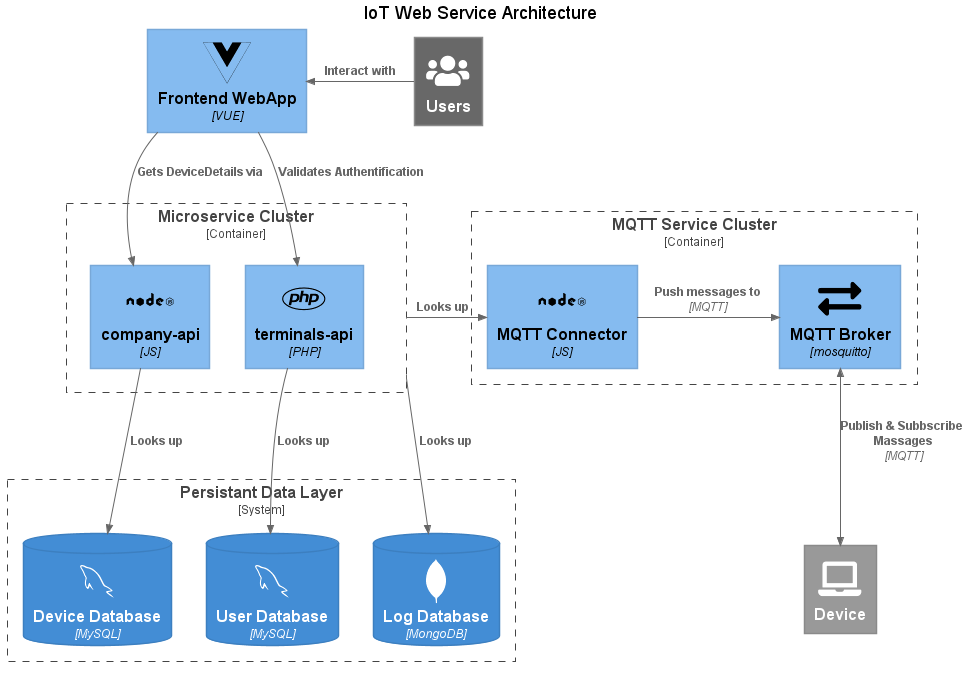
\includegraphics[width=.95\textwidth]{CCI-System-clean.png}
    \caption{IoT Web Service Architecture - [Alternative]}\label{fig::arch}
\end{figure} % Alternative
        \noindent As described above, the project used here is built on a microservice architecture. The advantage of this architecture is that it allows different technologies to be used for individual applications. Communication then takes place via a platform-independent protocol. If the load on a part of the application becomes critical, new instances of this application can simply be created and added to the service.\newline
        Figure~\ref{fig::arch} visualizes the architectural structure of the entire service. Users of this service only directly interact via the web interface (WebApp) with the segment of the system that is considered in this thesis.
        The web interface is created with the \ac{JS} framework Vue.js which generates a static bundle of HTML, CSS and \ac{JS} files which are served by a webserver. To access the system, users must authenticate themselves in the WebApp. This is done via a backend, written in PHP. In addition to authentication, this backend application also performs additional tasks which will be neglected in this work, for reasons of brevity. Provided the user is authenticated, the WebApp can display internal information and functions of all deployed \ac{IoT} devices. These dynamic information are provided by the NodeJS-based System-\ac{API}. All \ac{API} endpoints are implemented under the compliance with the \ac{OAS}. The \ac{OAS} allows for easy discoverability and understanding of the \ac{API} for humans and computers. It also provides versioning support of \ac{API}s to avoid unexpected errors in other applications. \newline
        Both, the authentication app and the System-\ac{API} have their own SQL databases that persistently provide relevant information. However, both applications write certain changes, made by the user, to a shared event database. MongoDB is used to provide schema flexible NoSQL database. To send specific instructions to, or receive information from a \ac{IoT} device, the system \ac{API} communicates with an MQTT-broker via the NodeJS-based MQTT-Connector. The MQTT-Connector provides an unified \ac{REST} \ac{API} for publishing and subscribing messages over the MQTT protocol. On a larger scale, the MQTT-Connector is used by several applications and is therefore a standalone application. Since only a part of this project is considered here, the System-\ac{API} is the only application communicating with the MQTT-Connector. The MQTT-broker exposes a public endpoint that offers various topics which devices can subscribe or publish to. Via this system the user can trigger a command in the web interface, which is then processed and logged by the system \ac{API}. Sequentially it is made available on the MQTT Broker via the MQTT-Connector. \ac{IoT} devices that have subscribed to the corresponding topic, receive this command and execute it. The result is published to another topic and can be accessed in the same way via the WebApp. Since the \ac{IoT} devices are connected to the Internet via SIM cards, and are therefore in an own restricted mobile carrier network, they are not directly accessible from the Internet. Through the described system, the IoT devices can execute commands from the outside without being accessible via the Internet.

        \subsubsection{Initial State of the Projects Development Environment}
        New developers joining the project have to clone all four repositories, install NodeJS 14, a specific version of the \ac{XAMPP} stack and must customize its configuration. Furthermore, the PHP project requires the package manager \wordhighlight{composer}, which must be installed separately. The configuration details must be taken from the documentation or are provided by a collaborator. To test the whole unified system developers also need to install a MQTT broker and the MongoDB database. Both applications need an initial administrator user which needs to be created, and the corresponding credentials need to be accessible by each \ac{API}. This is done by creating an \code{.env} file which is not tracked in the \ac{VCS}. Then a database and its schema must be created. Eventually network ports have to be adjusted and secrets for signing tokens have to be created.
        The access data for the databases must be created in each case, the ports of the individual applications must be coordinated and possibly secrets must be entered. These steps are necessary to just get the project running properly, the setup of developer tools like debugger has not been considered yet. Even in a small project this can take some time especially if one is not yet familiar with the project.\newline
        Even experienced project members experience challenges when working on such a project. Before the APIs can be launched, it must be ensured that the databases and other auxiliary tools are already running. To start all four applications (WebApp, Auth-backend, System-API, MQTT-Connector) a developer needs four terminal sessions or a terminal multiplexer to operate all applications. The program outputs (logs) are distributed over all four sessions and cannot be directly linked to each other, neither are they filterable nor searchable. When everything is running developers can now contribute value to the project. These restrictions would be acceptable as long as the work is not interrupted by a possible error case. A merge containing dependency or database schema updates by a team member can cause the environment of others to break. Error searching in very different setups is the result. The lack of consistent, reproducible setups is the cause for lasting troubleshooting sessions and the well-known iconic saying \textit{"But it works on my machine"}. This mirrors the problems of heterogeneous systems from section \ref{sec::problem}. It does not matter whether the individual development environments differ or the development environment to the production environment. The fact that there are always configuration differences is one root cause of before-mentioned problems. \newline
        These selected problems emerged in just one project. When working on multiple projects, the problem scope increases accordingly. Different databases, runtimes and dependencies further contribute to a greater potential for issues. The lack of project isolation may result in unintended side effects between projects that slow down the development process. To prevent these unnecessary slowdowns, the initial setup of an environment and its operation must be as homogeneous as possible.

        \subsubsection{Goal for the Target State}\label{sssec::goal}
        The goal is that by using DevContainers, a faster deployment of project environments is created that is common among all developers and has more similarity to the productive environment. This is made possible by the principle of virtualization, which provides a similar environment regardless of the host. Accordingly, this should avoid system-dependent errors and eliminate the lack of reproducibility. Thus, any system can be used as host operating system as long as it is supported by Docker. The DevContainer environment to be created is not intended to forcibly replace existing environments, but to provide an alternative solution that is also platform independent. New team members can quickly set up a working environment based either on Windows, Linux or macOS host, while offering an alternative for developers with existing environments that they can adapt too iteratively. Thus, a hybrid environment between the traditional development environments and DevContainer should be possible. Developers should continue to have free choice in their editors and utilities selection.\newline
        At any time, developers should be able to exercise control over the container runtime and the processes within the container. Thus, in the event of an error, they are independently able to replace a non-functioning container with a new one. The DevContainer environment should run locally and not require an internet connection to external servers in order to be unaffected by internet failures of external services. To ease the transition to a DevContainer based development environment it must be possible to set up the environment with a single command as well as to start all services with one command. Developers should not need to have explicit knowledge of how DevContainers work in order to use them.

    \subsection{Applying the DevContainer Approach}\label{ssec::apply}
    This section will apply the DevContainer concept described in section \ref{sec::solution_concept} to the Symbic project. First, the rough procedure of the process will be described, followed by the exact implementation and step-by-step descriptions. Problems, possible solutions and limitations of the concept will be described at the end.

        \subsubsection{Approach on the Project}\label{ssec::imp_approach}
        To provide a fully comprehensive development environment for all microservices of the Symbic project, each service will get its own DevContainer, as intended in a microservice architecture. This allows granular control over the individual services and makes it possible to implement a hybrid operation of traditionally running services and DevContainers. For this purpose, a \code{Dockerfile.dev} must be created for each service, which contains all the necessary runtime environments and other developer tools in a pre-build image. The program code is not copied into the container, but later included as bind-mount. This makes it possible to use any editor on the host without accidentally losing changes. Images have to be built less often and can be shared between applications with the same runtime. The orchestration of the individual services is then done with the Docker-Compose tool. Both the configuration all services and the Dockerfiles are then stored in \ac{VCS} according to the \ac{IaC} principle. Also, Docker-Compose creates persistent volumes mounts and bind-mounts from the host system. With the remote extension of \ac{VSCode}, developers can then attach themselves to any container process and take full control over the system and the running application.\newline
        Windows is used as the starting point for the development of the setup, as this is the most widely used operating system for development at Symbic. After the Docker images have been created and tested, they will later be automatically created by GitLab \ac{CI}. Once the setup is operational on Windows systems it is tested on other operating systems and adapted if necessary. Finally, scripts will be provided for the initial download of all repositories and the database initialization.

        \subsubsection{The Implementation Process}\label{ssec::imp_process}
        The next paragraphs will provide a step by step descriptions of how the DevContainer architecture was designed. Starting with the Dockerfiles for the images, over the creation of the \code{docker-compose.yml} file up to the usage of the environment via \ac{VSCode}.
        \myparagraph{Creating the Dockerfiles}
        The microservices project described in section \ref{ssec::project} are based on two technology stacks. The WebApp, the System-API and the MQTT-Connector are all based on the NodeJS runtime, where as the authentication backend is written in PHP. Accordingly, we need two variants of images. As already described in section \ref{sssec::docker}, Docker images are created from Dockerfiles. Each statement in a Dockerfile creates a new layer, this allows to build upon of already existing images.\newline
        As a basis for the nodejs based images the \code{mcr.microsoft.com/vscode/devcontainers/ javascript-node} image provided by Microsoft is used. This is a Debian based image which already comes with many developer tools and can be used without much modification. These Microsoft images were chosen because they are very similar to the production environment, come from a trusted source and are updated regularly. Upon this base additional tools like git, a ssh server, build tools and terminal editors vim and emacs are installed. As already stated, the program code is not written into the image, because it is mounted into the container via bind mount at runtime. The complete Dockerfile for the WebApp, the System-\ac{API} and the MQTT-Connector can be found in Listing \ref{code::docker_dev_node}.\newline
        However, for the PHP application, the Dockerfile is more complex. A Microsoft DevContainer image is again used as a starting point. It is especially built for PHP applications and ships with the Apache-\acs{HTTP}-Server and a package manager for installing PHP extensions. Line 2 in Listing \ref{code::docker_dev_php} specifies the PHP version that is used followed by the installation of several development tools. Subsequently, the PHP extensions used for the app and their dependencies are installed. Since this application also provides static assets, this time the source code is copied into the image followed by the installation of additional PHP packages using the PHP-Composer. In the last step the Apache web server is configured, and file permissions are adjusted. The image contains all needed resources in order to start the application and also includes several development tools such as the preconfigured \wordhighlight{Xdebug} debugger.\newline
        % !TeX root = ../thesis_main.tex

\begin{lstlisting}[language=docker, frame=single, caption={NodeJS DevContainer Dockerfile},label=code::docker_dev_node]
ARG NODE_VARIANT="14-buster"
FROM mcr.microsoft.com/vscode/devcontainers/javascript-node:
    ${NODE_VARIANT}

RUN apt-get update && apt-get install -y \
    git zsh ssh python3 make vim emacs
\end{lstlisting}

        For both the NodeJS image and the PHP image, the versions are passed as arguments. This makes it possible to influence the version of the used runtime when executing the build process. Thus, multiple images can be built from one Dockerfile without having to adapt it and developers have the possibility to adapt new runtimes without much effort. During the creation process, the images were created locally; in productive use, the GitLab \ac{CI} is responsible for creating regularly updated images. The job for creating the images is described in more detail at the end of this section.

        \myparagraph{Orchestrating the Microservices}
        The applications from the Symbic project in Figure \ref{fig::arch} need helper services. In order to work the project requires an SQL-Database, an MongoDB-Server and an MQTT-Broker. By choosing a MySQL-Server, the Eclipse-Mosquitto-Broker and the official MongoDB-Server, free pre-built official Docker images are available for all these applications. Listing \ref{code::compose_helper} shows how these services are configured in a \code{docker-compose.yml} file in order to be usable for other applications. Each application is defined as a service and with the corresponding Docker image it uses. To make the applications usable outside the virtual docker network, the internal network ports are exposed on the host system (see line 7, 16, 22 in Listing \ref{code::compose_helper}). To ensure that the data stored in the container is not lost when it is renewed, volumes are used to store application data persistently on the host. For this purpose, the name of the volume followed by the mount point of the volume in the container is specified in the volumes property. As typical for Docker, the configuration for the initial credentials is done via environment variables. In contrast, the Mosquitto-Server is configured by bind-mounting config files from the \code{manage-reop/config} folder to \code{mosquitto/config}. Eventually, the respective application ports are exposed on the host.\newline
        % !TeX root = ../thesis_main.tex

\begin{lstlisting}[language=docker-compose-2,caption={Auxiliary Services docker-compose.yml},breaklines=true,label={code::compose_helper}]
version: "3"
services:
  db:
    image: mysql
    environment:
      - MYSQL_ROOT_PASSWORD=yes
    ports:
      - 3306:3306
    volumes:
      - db_sql_data:/var/lib/mysql

  mongo:
    image: mongo:4.4-focal
    environment:
      - MONGO_INITDB_ROOT_USERNAME=root
      - MONGO_INITDB_ROOT_PASSWORD=none
      - MONGO_INITDB_DATABASE=dm-cu-local
    ports:
      - 27017:27017
    volumes:
      - db_mongo_data:/data/db

  mosquitto:
    image: eclipse-mosquitto
    ports:
      - 1883:1883
    volumes:
        - mosquitto_data:/mosquitto/data
        - ./manage-reop/config:/mosquitto/config
\end{lstlisting}

        Without applying the concept of actual DevContainers, the configuration in Listing \ref{code::compose_helper} already enriches the developer experience. Developers do not have to install and configure extra programs such as databases, but can make them available quickly, uniformly and platform-independently with one command.\newline
        In order to use DevContainers, the individual applications also must be defined as services. Listing \ref{code::compose_service} shows this as an example for the System-\ac{API}. The name of the DevContainer image is used as a starting point just like in the previous section \ref{sec::solution_concept}. Subsequently, the credentials for the auxiliary services are made available to the application via environment variables. Since the source code is not within the container this is mapped by a bind-mount into the container. Now all the necessary requirements for starting the application in the DevContainer are available.\newline
        Since the project is a NodeJS application, all dependencies are stored locally in the program directory under the \code{node\_modules} folder. These dependencies are operating system specific, for this reason it can happen that the NodeJS application does not start when developing on a Windows host while the DevContainer is based on Linux. Developers would have to delete and reinstall all dependencies whenever the DevContainer is not in use. However, this can be avoided by using the Docker overlay file system. A volume managed by docker is created, which overlays the local dependencies mapped via a bide-mount (see line 17 in Listing \ref{code::compose_service}). This makes all dependencies used within  the DevContainer independent of those installed locally. For other programming languages that do not store their dependencies in the project directory, this does not need to be done. A volume is also used for the extensions installed by VSCode, this avoids that extensions have to be reinstalled every time the image is updated.\newline
        % !TeX root = ../thesis_main.tex

\begin{lstlisting}[language=docker-compose-2,caption={Auxiliary Services \code{docker-compose.yml}},breaklines=true,label={code::compose_service}]
services:                       # Exemplary service
  system-api:                   # configuration
    image: system-api/dev-container
    entrypoint: "/workspace/.devcontainer/entrypoint.sh"
    environment:                # Configure settings
      - PORT=8090               # for auxiliary services
      - MONGO_DB_HOST=mongo
      - MONGO_DB_USER=root
      - MONGO_DB_PW=none
      - SQL_HOST=db
      - SQL_USER=root
      - SQL_PASSWORD=yes
      - SQL_DB_NAME=local-device-db
    volumes:
      - ./system-api:/workspace
      - system_api_node_modules:/workspace/node_modules
      - vscode_extentions:/root/.vscode-server/extensions
    ports:
      - 8090:8090
volumes:                        # Persistent storage
  system_api_node_modules:      # managed by Docker
  vscode_extentions:
\end{lstlisting}

        When the service is started, its entrypoint is executed. For the NodeJS applications, this is a script similar to Listing \ref{code::entry} that installs all the necessary dependencies via npm, if they are not already present, and then starts the application in development mode via nodemon. The complete \code{docker-compose.yml} file with all application services and auxiliary services can be found in the appendix under Listing \ref{code::compose_service_all}.
    \begin{lstlisting}[language=bash,caption={DevContainer \code{entryscript.sh}},breaklines=true,label={code::entry}]
#!/bin/bash
NODE_MODULES=/workspace/node_modules && cd /workspace

# Check if modules are present
if [ -z "$(ls -A ${NODE_MODULES})" ]; then
    npm i
fi

# Start the main process in background & remember the pid
./node_modules/.bin/nodemon index.js&
MAIN_PROCESS_PID=$!

echo -n $MAIN_PROCESS_PID > /tmp/pid.tmp
while sleep 1000; do :; done
        \end{lstlisting}
        \myparagraph{Enabeling Development}
        Following the procedure above, all applications are started in development mode without the need to open an editor. Changes on the code, by any editor on the host, directly apply to all NodeJS application since \wordhighlight{nodemon} enables hot-code-reloading. This may not be possible in every programming language and is not certainly supported by compiled languages.\newline
        If the developer wants to have more control over the application he can open the application in the DevContainer via \ac{VSCode}. On startup \ac{VSCode} terminates the previously automatically started process via the \ac{PID} and the developer now has complete control over the application via the built-in terminal. However, in order for the container not to terminate as intended when the main process terminates, a process must continue to run to keep the container alive. For this reason the entryscript executes an infinite loop at the end. To determine the container which \ac{VSCode} connects to, a \code{devcontainer.json} file is required. Listing \ref{code::devcontainer_json} shows auch a \code{devcontainer.json} file. It must exist for each application, developers work on and defines the service that is worked on. The development process compared to a local \ac{VSCode} instance does not differ.
        \myparagraph{Combination of all Components}
        Docker provides the virtualization of the runtime, Docker-Compose orchestrates the individual services, enables the integration of local code and \ac{VSCode} offers a comfortable user interface. In order for the directories to be integrated accordingly, it is imperative to adhere to a certain project structure that is the same for all developers. Only then the relative paths of the bind-mounts can be applied automatically. For the Symbic project, the directory structure can be found in the appendix in figure \ref{fig::dirstructure}. All projects are arranged in subfolders, the \code{docker-compose.yml} file is made available as a system-link from the management repro. To support the architecture under Linux it was only necessary to make sure that all files are checked out with the correct line ending and that the appropriate Linux function is used to create a system-link.\newline
        Configuration files which are project-specific are stored in a management repository. It also contains handy scripts to perform operations on several repositories at once and sets initial configuration. The GitLab \ac{CI} automatically creates all needed Docker images and provides them via a private registry. Listing \ref{code::ci_build_yml} shows a \code{.gitlab-ci.yml} file for \ac{CI} configuration using the \wordhighlight{kaniko} executor to build docker images. The executor is told the repository context, the Dockerfile, the line location and which variant of the container is being built. The build is executed on every push-event to the GitLab repository.\newline
        By adding a logging parameter to the \code{docker-compose.yml} file, all application logs can also be sent to any system and displayed graphically. In this concept, a Grafana container is used that gets its logs from the \wordhighlight{Loki} log-shipper via a Docker plugin.\newline
        % !TeX root = ../thesis_main.tex

\begin{lstlisting}[language=yml,caption={GitLab \ac{CI} build file for Docker Images},breaklines=true,label={code::ci_build_yml}]
build_dev_container:
  stage: build
  image:
    name: gcr.io/kaniko-project/executor:debug
  variables:
    DOCKERFILE: $CI_PROJECT_DIR/.devcontainer/Dockerfile.dev
    BUILD_IMAGE_TAG: $CI_REGISTRY_IMAGE/dev-container:latest
    NODE_VARIANT: 14-buster-slim
  script:
    - /kaniko/executor --context $CI_PROJECT_DIR
    --build-arg NODE_VARIANT=$NODE_VARIANT
    --dockerfile $DOCKERFILE
    --destination $BUILD_IMAGE_TAG
  rules:
      - if: $CI_COMMIT_BRANCH == "master"

\end{lstlisting}


        \subsubsection{Encountered Challenges and Limitations}
        During the creation of the DevContainer architecture some challenges arose similar to the problems described in section \ref{sec::problem}. The biggest challenge was the differences between a Windows and a Linux based system. Since the source code is mapped into the container via bind-mounts and not bundled within the image, all mounted files have the \code{CR} line ending. Linux programs like Bash and \ac{SSH} can't read this format, therefore their execution fails. Creating an \code{.gitatrubtes} file with the following content solves the problem.
        \begin{lstlisting}[language=yml,frame=none, numbers=none, backgroundcolor=\color{codebg}]
* text=auto eol=lf
*.{cmd,[cC][mM][dD]} text eol=crlf
*.{bat,[bB][aA][tT]} text eol=crlf
        \end{lstlisting}
        \vspace{-0.5cm}
        All files (except \code{.bat}/\code{.cmd} scripts) will be checked out with the Linux \code{LF} line ending. These are supported by most editors including Windows focused editors.\newline
        Another challenge was the lack of isolation of local NodeJS dependencies. Deleting the \code{node\_modules} folder and reinstalling all dependencies is not a reasonable solution in case developers switch between the local- or the DevContainer environment. The overlay file system can overshadow individual folders or files that are mounted via bind-mount. This way operating system specific files can be isolated. However, the use of non-Linux oriented file systems brings some problems. The NodeJS applications use nodemon to reload the application whenever file changes are made, in order to apply changes immediately. Nodemon monitors the file system for changes, just like other hot-reloading solutions. However, due to the fundamental differences between an NTFS file system and the Docker overlay file system, this monitoring does not work by default. To enable this feature, an additional parameter must be specified so that nodemon actively polls for changes. With this parameter, hot-reloading works, but requieres more processing power for active file-polling.\newline
        To make the usage of DevContainer as comfortable as possible all applications are started with the container start likewise. However, since Docker containers only run until their initial process is terminated, a wrapper had to be created that starts the application process but does not terminate when the developer takes control of the application. Listing \ref{code::entry} shows how this was possible with a short Bash script. The application process is started in the background while the main process is an infinite loop. \newline
        Depending on the project, different technologies are used which come with different requirements and challenges. This can be seen in the very simple Dockerfile for the NodeJS application while the Dockerfile for the PHP application is much more complex. When using other technologies, the implementation will have to be adapted accordingly.\newline
        Although there have been challenges in the creation of the architecture and the individual services, these has been largely solved by minor adjustments. However, the additional load due to containerization could not be solved. Under Windows, the entire Linux kernel has to be virtualized. For the conversion of file accesses from between Docker and Windows, further load applies. This is even amplified by the active searching of file change ends by nodemon. \acs{I/O} heavy tasks like installing many \code{node\_modules} cause a noticeable overhead on the system. The more applications and the more demanding the applications are, the greater the added overhead and load on the system. The impact of this drawback is further described in section \ref{sec::eval}. \newline
        During development, bugs have also been encountered when using Docker Desktop on Windows. A memory leak caused the system memory to reach capacity when Docker images where created repeatedly. Although this can be prevented by a setting on the \ac{WSL} system, it is not a permanent solution to the problem. Also, Docker Inc. changed their licensing model for Docker Desktop during the writing of this paper, so that now its only free of charge by companies with less than 250 employees and less than \$10 million in revenue \cite{dockerblog}. However, this does not apply to Docker Community Edition for Linux.

        \subsection{Final State}\label{sec::final}
        The newly created Development environment provides a uniform environment across multiple systems regarding the operating system used. Thanks to virtualization, the greatest possible similarity between the proposed environment and productive environments is achieved. Auxiliary processes no longer have to be created and configured individually as their definitions are available pre-configured in the repository. Through the use of Docker, programs are also available under Windows and macOS that were previously only available under Linux. By aligning the environment through virtualization, configuration-related errors become traceable and can be avoided. \newline
        Developers are not compelled to use the new DevContainer environment as it has been achieved to isolate both environments from each other. Subsequently, individual applications can be extended using the DevContainer solution. The command \code{docker-compose up service\_1 service\_2 \ldots service\_n } starts only the explicitly specified applications as a container while all other applications can still be run locally. Explicit changes to the applications for the use of the DevContainer were not necessary.\newline
        However, a noticeable overhead due to the use of the DevContainer was noticed during use, especially under Windows. The effects of this additional load are discussed in the next section along with the advantages of the DevContainer environment.

